\documentclass{scrartcl}
\usepackage[utf8]{inputenc} 
\usepackage[T1]{fontenc} 
\usepackage[dvipsnames]{xcolor} 
\usepackage[object=vectorian]{pgfornament}
\usetikzlibrary{calc}
\definecolor{fondpaille}{cmyk}{0,0,0.1,0}

\begin{document}
\pagecolor{fondpaille}
\color{Maroon} 
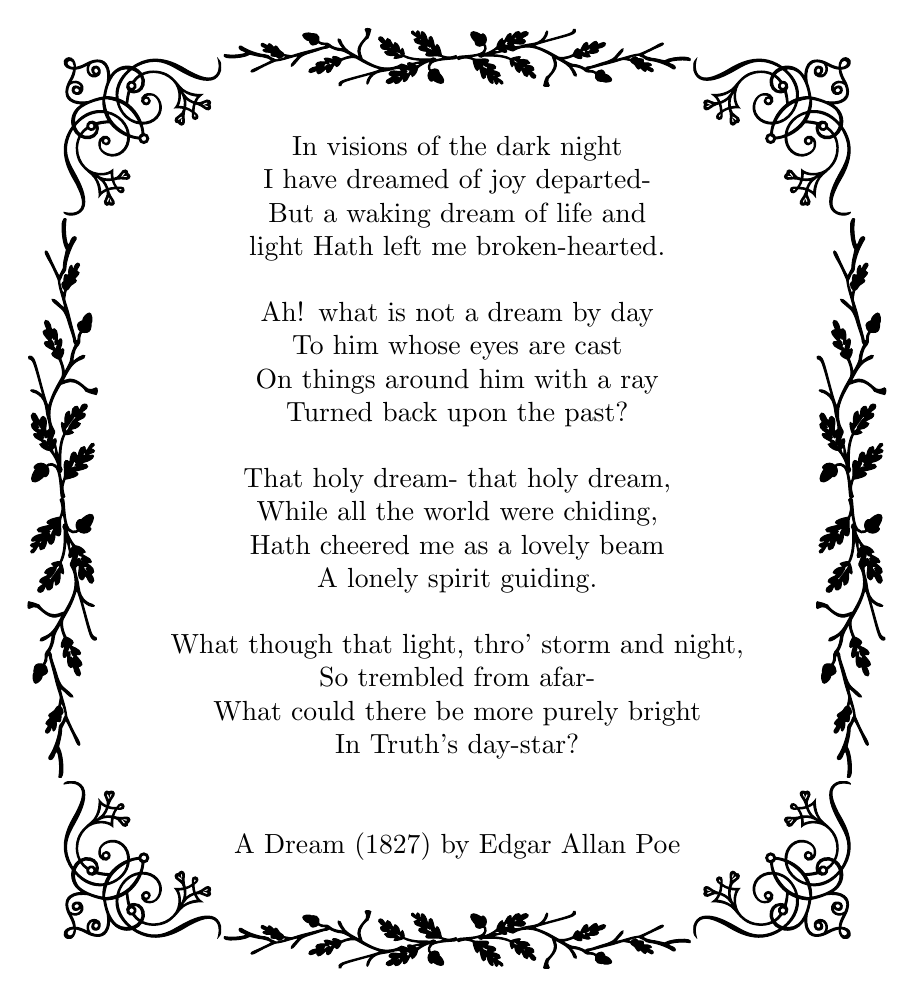
\begin{tikzpicture}[every node/.style={inner sep=0pt}]   
\node[text width=8cm,align=center](Text){%
In visions of the dark night\\
I have dreamed of joy departed-\\
But a waking dream of life and light\
Hath left me broken-hearted.\\
\bigskip
Ah! what is not a dream by day\\
To him whose eyes are cast \\
On things around him with a ray \\
Turned back upon the past? \\
\bigskip        
That holy dream- that holy dream,\\
While all the world were chiding,\\
Hath cheered me as a lovely beam\\
A lonely spirit guiding.\\
\bigskip        
What though that light, thro' storm and night,\\
So trembled from afar- \\
What could there be more purely bright \\
In Truth's day-star? \\
\vspace{24pt}
 A Dream  (1827) by Edgar Allan Poe 
} ;
\node[shift={(-1cm,1cm)},anchor=north west](CNW)  at (Text.north west)
	             {\pgfornament[width=2cm]{61}};
\node[shift={(1cm,1cm)},anchor=north east](CNE)   at (Text.north east)
	             {\pgfornament[width=2cm,symmetry=v]{61}}; 
\node[shift={(-1cm,-1cm)},anchor=south west](CSW) at (Text.south west)
	             {\pgfornament[width=2cm,symmetry=h]{61}}; 
\node[shift={(1cm,-1cm)},anchor=south east](CSE)  at (Text.south east)   
	             {\pgfornament[width=2cm,symmetry=c]{61}};  
\pgfornamenthline{CNW}{CNE}{north}{87}
\pgfornamenthline{CSW}{CSE}{south}{87}
\pgfornamentvline{CNW}{CSW}{west}{87}
\pgfornamentvline{CNE}{CSE}{east}{87} 
\end{tikzpicture}
\end{document}

                       